% Compile with: pdflatex mindmap.tex
\documentclass[border=15mm]{standalone}
\usepackage[T1]{fontenc}
\usepackage{lmodern}
\usepackage{tikz}
\usetikzlibrary{mindmap,backgrounds,positioning}

% --- Color palette ---
\definecolor{coreColor}{HTML}{495057}
\definecolor{brA}{HTML}{E8590C}  % Orange  - Generative Design
\definecolor{brB}{HTML}{1971C2}  % Blue    - Property Prediction
\definecolor{brC}{HTML}{2F9E44}  % Green   - Formulation Optimization
\definecolor{brD}{HTML}{9C36B5}  % Purple  - Autonomous Experimentation
\definecolor{brE}{HTML}{E67700}  % Amber   - Multifunctional Properties
\definecolor{brF}{HTML}{0CA678}  % Teal    - Foundation Models
\definecolor{brG}{HTML}{D6336C}  % Pink    - Process & Quality Control

\begin{document}
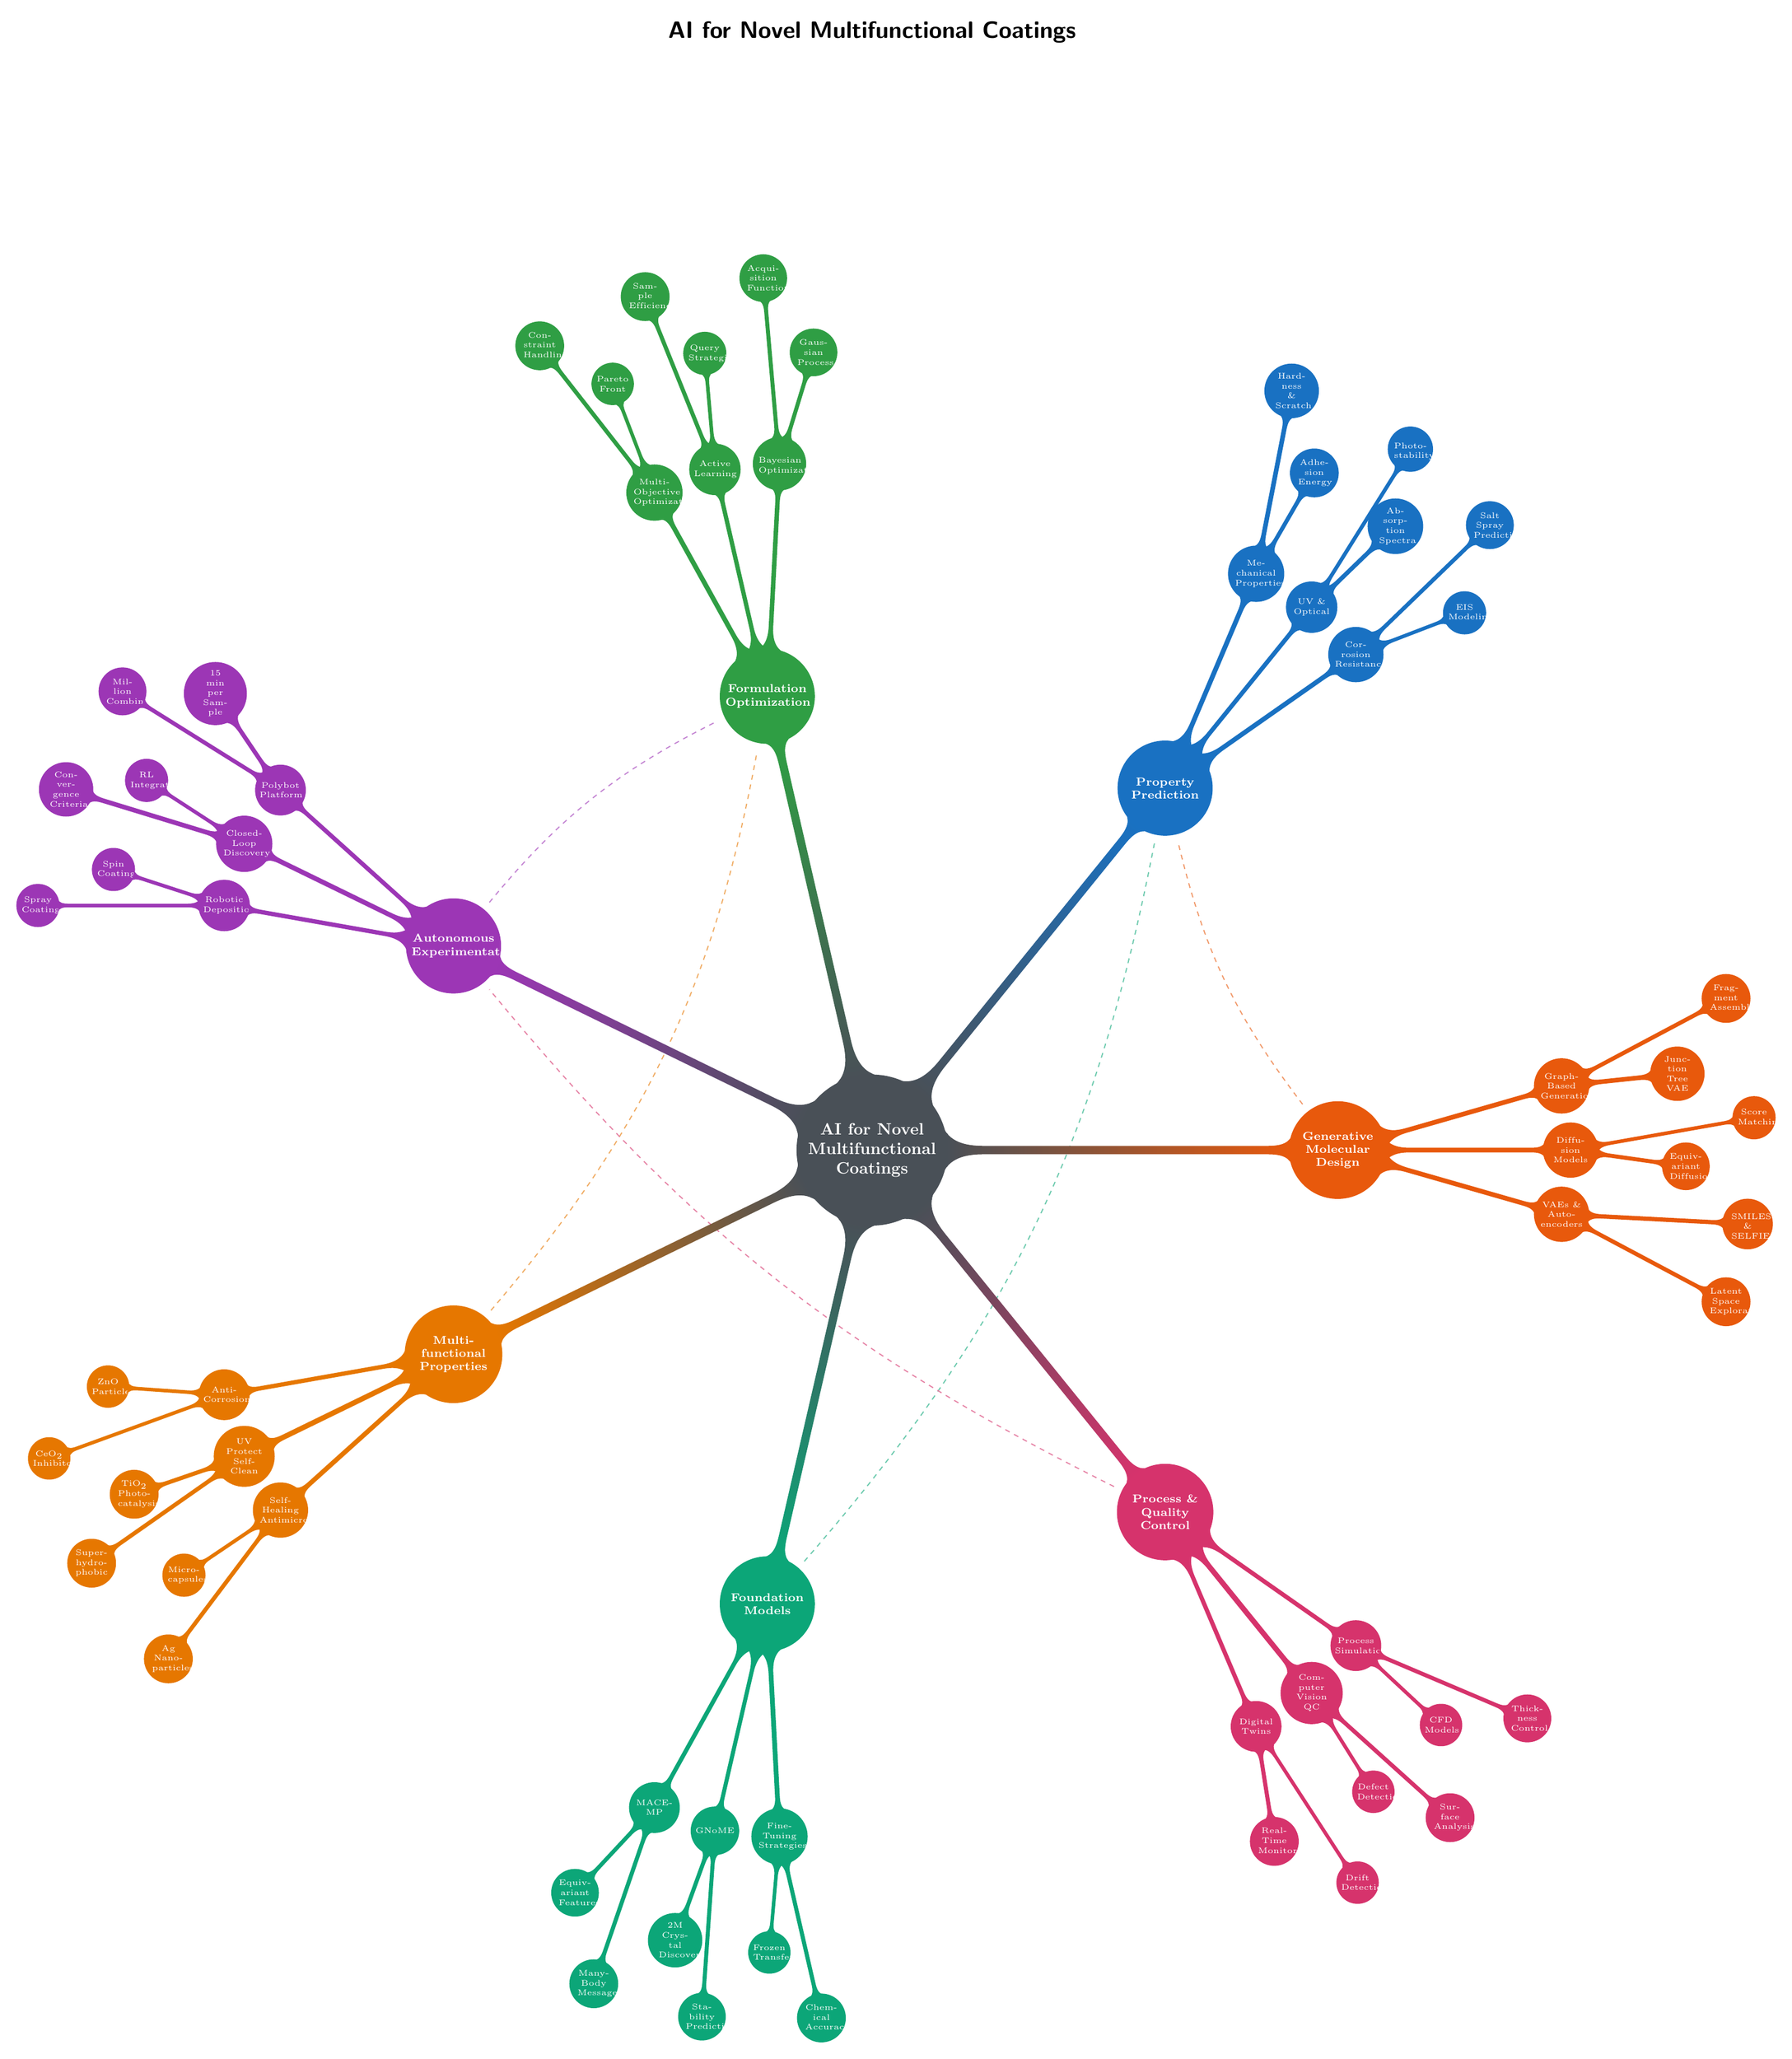
\begin{tikzpicture}

% --- Title ---
\node[font=\Large\bfseries\sffamily] at (0,24)
  {AI for Novel Multi\-functional Coatings};

\begin{scope}[
  mindmap,
  every node/.style={concept, execute at begin node=\hskip0pt},
  grow cyclic,
  text=white,
  concept color=coreColor,
  level 1/.append style={
    level distance=10cm, sibling angle=51,
    font=\scriptsize\bfseries, minimum size=2.0cm, text width=1.8cm,
  },
  level 2/.append style={
    level distance=5.0cm, sibling angle=16,
    font=\tiny, minimum size=1.0cm, text width=0.9cm,
  },
  level 3/.append style={
    level distance=4.0cm, sibling angle=25,
    font=\tiny, minimum size=0.8cm, text width=0.7cm,
  },
]

\node [font=\normalsize\bfseries, minimum size=3.2cm, text width=2.8cm]
  (center) {AI for Novel\\Multi\-functional\\Coatings}
%
% ===== Branch 1: Generative Molecular Design (0 deg) =====
  child [concept color=brA, grow=0] {
    node (gendesign) {Generative\\Molecular\\Design}
    child [grow=-16] {
      node {VAEs \&\\Auto\-encoders}
      child [grow=-28, level distance=4.0cm] { node {Latent Space\\Exploration} }
      child [grow=-3, level distance=4.0cm] { node {SMILES \&\\SELFIES} }
    }
    child [grow=0] {
      node {Diffusion\\Models}
      child [grow=-8, level distance=2.5cm] { node {Equivariant\\Diffusion} }
      child [grow=10, level distance=4.0cm] { node {Score\\Matching} }
    }
    child [grow=16] {
      node {Graph-Based\\Generation}
      child [grow=6, level distance=2.5cm] { node {Junction\\Tree VAE} }
      child [grow=28, level distance=4.0cm] { node {Fragment\\Assembly} }
    }
  }
%
% ===== Branch 2: Property Prediction (51 deg) =====
  child [concept color=brB, grow=51] {
    node (proppred) {Property\\Prediction}
    child [grow=35] {
      node {Corrosion\\Resistance}
      child [grow=21, level distance=2.5cm] { node {EIS\\Modeling} }
      child [grow=44, level distance=4.0cm] { node {Salt Spray\\Prediction} }
    }
    child [grow=51] {
      node {UV \&\\Optical}
      child [grow=44, level distance=2.5cm] { node {Absorption\\Spectra} }
      child [grow=58, level distance=4.0cm] { node {Photo\-stability} }
    }
    child [grow=67] {
      node {Mechanical\\Properties}
      child [grow=60, level distance=2.5cm] { node {Adhesion\\Energy} }
      child [grow=79, level distance=4.0cm] { node {Hardness \&\\Scratch} }
    }
  }
%
% ===== Branch 3: Formulation Optimization (103 deg) =====
  child [concept color=brC, grow=103] {
    node (formulopt) {Formulation\\Optimization}
    child [grow=87] {
      node {Bayesian\\Optimization}
      child [grow=73, level distance=2.5cm] { node {Gaussian\\Process} }
      child [grow=95, level distance=4.0cm] { node {Acquisition\\Functions} }
    }
    child [grow=103] {
      node {Active\\Learning}
      child [grow=95, level distance=2.5cm] { node {Query\\Strategies} }
      child [grow=112, level distance=4.0cm] { node {Sample\\Efficiency} }
    }
    child [grow=119] {
      node {Multi-Objective\\Optimization}
      child [grow=111, level distance=2.5cm] { node {Pareto\\Front} }
      child [grow=128, level distance=4.0cm] { node {Constraint\\Handling} }
    }
  }
%
% ===== Branch 4: Autonomous Experimentation (154 deg) =====
  child [concept color=brD, grow=154] {
    node (autoexp) {Autonomous\\Experimentation}
    child [grow=138] {
      node {Polybot\\Platform}
      child [grow=124, level distance=2.5cm] { node {15 min\\per Sample} }
      child [grow=148, level distance=4.0cm] { node {Million\\Combinations} }
    }
    child [grow=154] {
      node {Closed-Loop\\Discovery}
      child [grow=147, level distance=2.5cm] { node {RL\\Integration} }
      child [grow=163, level distance=4.0cm] { node {Convergence\\Criteria} }
    }
    child [grow=170] {
      node {Robotic\\Deposition}
      child [grow=162, level distance=2.5cm] { node {Spin\\Coating} }
      child [grow=180, level distance=4.0cm] { node {Spray\\Coating} }
    }
  }
%
% ===== Branch 5: Multifunctional Properties (206 deg) =====
  child [concept color=brE, grow=206] {
    node (multifunc) {Multi\-functional\\Properties}
    child [grow=190] {
      node {Anti-\\Corrosion}
      child [grow=176, level distance=2.5cm] { node {ZnO\\Particles} }
      child [grow=200, level distance=4.0cm] { node {CeO$_2$\\Inhibitors} }
    }
    child [grow=206] {
      node {UV Protect\\Self-Clean}
      child [grow=199, level distance=2.5cm] { node {TiO$_2$\\Photo\-catalysis} }
      child [grow=215, level distance=4.0cm] { node {Super\-hydro\-phobic} }
    }
    child [grow=222] {
      node {Self-Healing\\Antimicrobial}
      child [grow=214, level distance=2.5cm] { node {Micro\-capsules} }
      child [grow=233, level distance=4.0cm] { node {Ag Nano\-particles} }
    }
  }
%
% ===== Branch 6: Foundation Models (257 deg) =====
  child [concept color=brF, grow=257] {
    node (foundmod) {Foundation\\Models}
    child [grow=241] {
      node {MACE-MP}
      child [grow=227, level distance=2.5cm] { node {Equivariant\\Features} }
      child [grow=251, level distance=4.0cm] { node {Many-Body\\Messages} }
    }
    child [grow=257] {
      node {GNoME}
      child [grow=250, level distance=2.5cm] { node {2M Crystal\\Discoveries} }
      child [grow=266, level distance=4.0cm] { node {Stability\\Prediction} }
    }
    child [grow=273] {
      node {Fine-Tuning\\Strategies}
      child [grow=265, level distance=2.5cm] { node {Frozen\\Transfer} }
      child [grow=283, level distance=4.0cm] { node {Chemical\\Accuracy} }
    }
  }
%
% ===== Branch 7: Process & Quality Control (309 deg) =====
  child [concept color=brG, grow=309] {
    node (processqc) {Process \&\\Quality Control}
    child [grow=293] {
      node {Digital\\Twins}
      child [grow=279, level distance=2.5cm] { node {Real-Time\\Monitoring} }
      child [grow=303, level distance=4.0cm] { node {Drift\\Detection} }
    }
    child [grow=309] {
      node {Computer\\Vision QC}
      child [grow=302, level distance=2.5cm] { node {Defect\\Detection} }
      child [grow=318, level distance=4.0cm] { node {Surface\\Analysis} }
    }
    child [grow=325] {
      node {Process\\Simulation}
      child [grow=317, level distance=2.5cm] { node {CFD\\Models} }
      child [grow=337, level distance=4.0cm] { node {Thickness\\Control} }
    }
  }
;
\end{scope}

% --- Cross-branch connections ---
\begin{pgfonlayer}{background}
  % Generative Design <-> Property Prediction (molecules need property validation)
  \draw [dashed, brA!60, line width=0.7pt, shorten >=6pt, shorten <=6pt]
    (gendesign) to[bend left=12] (proppred);
  % Autonomous Experimentation <-> Formulation Optimization (robots implement BO)
  \draw [dashed, brD!60, line width=0.7pt, shorten >=6pt, shorten <=6pt]
    (autoexp) to[bend left=12] (formulopt);
  % Foundation Models <-> Property Prediction (pre-trained models enable prediction)
  \draw [dashed, brF!60, line width=0.7pt, shorten >=6pt, shorten <=6pt]
    (foundmod) to[bend right=15] (proppred);
  % Multifunctional Properties <-> Formulation Optimization (target props drive optimization)
  \draw [dashed, brE!60, line width=0.7pt, shorten >=6pt, shorten <=6pt]
    (multifunc) to[bend right=15] (formulopt);
  % Process & QC <-> Autonomous Experimentation (digital twins guide lab automation)
  \draw [dashed, brG!60, line width=0.7pt, shorten >=6pt, shorten <=6pt]
    (processqc) to[bend left=12] (autoexp);
\end{pgfonlayer}

\end{tikzpicture}
\end{document}
